\documentclass[12pt,a4paper]{article}

% ─── Page Layout ───────────────────────────────────────────────────────────────
\usepackage[a4paper, margin=0.8in, headheight=14pt]{geometry}

% ─── Fonts (XeLaTeX) ───────────────────────────────────────────────────────────
\usepackage{fontspec}
\usepackage{unicode-math}
\setmainfont{TeX Gyre Pagella}
\setmonofont[Scale=0.88]{TeX Gyre Cursor}
\setmathfont{Latin Modern Math}

% ─── Packages ──────────────────────────────────────────────────────────────────
\usepackage{xcolor}
\usepackage{colortbl}
\usepackage{titlesec}
\usepackage{enumitem}
\usepackage{tabularx}
\usepackage{booktabs}
\usepackage{array}
\usepackage{amsmath}
\usepackage{tikz}
\usetikzlibrary{shapes.geometric, arrows.meta, positioning, calc, fit, decorations.pathreplacing, patterns}
\usepackage{tcolorbox}
\tcbuselibrary{skins, breakable}
\usepackage{hyperref}
\usepackage{fancyhdr}
\usepackage{graphicx}
\usepackage{microtype}
\hyphenpenalty=10000
\exhyphenpenalty=10000
\sloppy
\usepackage{caption}
\usepackage{setspace}
\usepackage{multirow}
\usepackage{tocloft}

% ─── Q&A helper ────────────────────────────────────────────────────────────────
\newcommand{\Q}[1]{\textbf{#1}\par\noindent\ignorespaces}

% ─── Colour Palette ────────────────────────────────────────────────────────────
\definecolor{myred}{RGB}{196,30,58}
\definecolor{mydark}{RGB}{30,30,50}
\definecolor{mygreen}{RGB}{14,120,80}
\definecolor{myteal}{RGB}{0,130,140}
\definecolor{myamber}{RGB}{180,100,0}
\definecolor{mypurple}{RGB}{100,30,160}
\definecolor{mygray}{RGB}{246,247,249}
\definecolor{mgframe}{RGB}{180,185,200}
\definecolor{watermark}{RGB}{145,150,170}
\definecolor{hdrred}{RGB}{250,232,235}
\definecolor{hdrgreen}{RGB}{220,244,233}
\definecolor{hdrteal}{RGB}{220,242,244}
\definecolor{hdramber}{RGB}{253,242,215}
\definecolor{hdrpurple}{RGB}{238,228,255}
\definecolor{hdrgray}{RGB}{238,240,245}
\definecolor{rowalt}{RGB}{250,251,253}

% ─── Section Formatting ────────────────────────────────────────────────────────
\titleformat{\section}
  {\large\bfseries\color{myred}}{\thesection.}{0.5em}{}
  [\vspace{1pt}{\color{myred}\rule{\linewidth}{0.8pt}}]
\titleformat{\subsection}
  {\normalsize\bfseries\color{myteal}}{\thesubsection}{0.5em}{}
\titlespacing*{\section}{0pt}{18pt}{7pt}
\titlespacing*{\subsection}{0pt}{11pt}{4pt}

% ─── Paragraph ─────────────────────────────────────────────────────────────────
\setlength{\parindent}{0pt}
\setlength{\parskip}{4pt}

% ─── TOC Styling ───────────────────────────────────────────────────────────────
\renewcommand{\cfttoctitlefont}{\large\bfseries\color{myred}}
\renewcommand{\cftaftertoctitle}{\par\noindent{\color{myred}\rule{\linewidth}{0.8pt}}}
\setlength{\cftbeforetoctitleskip}{0pt}
\setlength{\cftaftertoctitleskip}{6pt}
\renewcommand{\cftsecfont}{\normalsize\bfseries\color{mydark}}
\renewcommand{\cftsecpagefont}{\normalsize\bfseries\color{mydark}}
\renewcommand{\cftsecleader}{\cftdotfill{\cftdotsep}}
\setlength{\cftbeforesecskip}{7pt}
\renewcommand{\cftsubsecfont}{\small\color{mydark}}
\renewcommand{\cftsubsecpagefont}{\small\color{mydark}}
\setlength{\cftbeforesubsecskip}{3pt}
\setlength{\cftsubsecindent}{1.4em}

% ─── Table helpers ─────────────────────────────────────────────────────────────
\renewcommand{\arraystretch}{1.45}
\setlength{\tabcolsep}{6pt}
\arrayrulecolor{mydark}
\newcolumntype{B}[1]{>{\small\bfseries\raggedright\arraybackslash}m{#1}}
\newcolumntype{Y}{>{\small\raggedright\arraybackslash}X}
\renewcommand{\tabularxcolumn}[1]{m{#1}}

% ─── Header / Footer ───────────────────────────────────────────────────────────
\pagestyle{fancy}
\fancyhf{}
\fancyhead[L]{\small\color{myred}\textbf{EC302}\;\color{mydark}--- Digital System Design}
\fancyhead[R]{\small\color{myteal}\textbf{Module 3 Notes}}
\fancyfoot[C]{\small\color{mydark}\thepage}
\fancyfoot[R]{\small\color{watermark}\textit{\copyright\ Biraj}}
\renewcommand{\headrulewidth}{0.5pt}
\renewcommand{\footrulewidth}{0.3pt}

% ─── Hyperref ──────────────────────────────────────────────────────────────────
\hypersetup{
  colorlinks=true, linkcolor=myteal, urlcolor=myteal,
  pdfauthor={Biraj Sarkar (CGEC)},
  pdftitle={EC302 --- Module 3 Notes: Logic Families, Memories, PLDs, ADCs, and DACs}
}

% ─── tcolorbox styles ──────────────────────────────────────────────────────────
\tcbset{
  tikzbox/.style={
    colback=mygray, colframe=mgframe, boxrule=0.6pt, arc=4pt,
    left=8pt, right=8pt, top=6pt, bottom=6pt,
    colbacktitle=mgframe, coltitle=mydark,
    fonttitle=\small\bfseries
  },
  defbox/.style={
    colback=hdrgreen, colframe=mygreen, boxrule=0.8pt, arc=4pt,
    left=9pt, right=9pt, top=6pt, bottom=6pt,
    colbacktitle=mygreen, coltitle=white,
    fonttitle=\small\bfseries
  },
  formulabox/.style={
    colback=hdrteal, colframe=myteal, boxrule=0.8pt, arc=4pt,
    left=9pt, right=9pt, top=6pt, bottom=6pt,
    colbacktitle=myteal, coltitle=white,
    fonttitle=\small\bfseries
  },
  examplebox/.style={
    colback=hdramber, colframe=myamber, boxrule=0.8pt, arc=4pt,
    left=9pt, right=9pt, top=6pt, bottom=6pt,
    colbacktitle=myamber, coltitle=white,
    fonttitle=\small\bfseries
  },
  masonbox/.style={
    colback=hdrpurple, colframe=mypurple, boxrule=0.8pt, arc=4pt,
    left=9pt, right=9pt, top=6pt, bottom=6pt,
    colbacktitle=mypurple, coltitle=white,
    fonttitle=\small\bfseries
  },
  exambox/.style={
    colback=hdrpurple, colframe=mypurple, boxrule=1pt, arc=5pt,
    left=10pt, right=10pt, top=8pt, bottom=8pt,
    colbacktitle=mypurple, coltitle=white,
    fonttitle=\bfseries,
    breakable, title after break={\textbf{Frequently Asked / Viva Questions (contd.)}}
  }
}

\tcbset{after={\color{black}}}

% ─── TikZ styles ───────────────────────────────────────────────────────────────
\tikzset{
  sysblock/.style={rectangle, draw=myteal, fill=hdrteal,
    minimum width=2.2cm, minimum height=1.3cm,
    font=\small\bfseries, rounded corners=3pt, line width=0.8pt, align=center},
  logicnode/.style={rectangle, draw=mypurple, fill=hdrpurple,
    minimum width=2.0cm, minimum height=1.2cm,
    font=\small\bfseries, rounded corners=3pt, line width=0.8pt, align=center},
  resnode/.style={rectangle, draw=mydark, fill=white,
    minimum width=1.0cm, minimum height=0.6cm,
    font=\scriptsize\bfseries, line width=0.6pt, align=center},
  flowarrow/.style={-Stealth, thick, color=mydark}
}

\begin{document}

% ─── Title Page ───────────────────────────────────────────────────────────────
\begin{titlepage}
  \centering
  \vspace*{1.5cm}
  {\Huge\bfseries\color{myred} Digital System Design\par}
  \vspace{0.4cm}
  {\LARGE\bfseries\color{myteal} Module 3 --- Logic Families, Semiconductor Memories, PLDs, ADCs, and DACs\par}
  \vspace{0.8cm}
  {\large\textbf{Course Code:} EC302 \;\textbar\; \textbf{Semester:} 3rd Semester (ECE)\par}
  \vspace{0.2cm}
  {\large MAKAUT B.Tech Maulana Abul Kalam Azad University of Technology\par}
  \vspace{1.5cm}

  \begin{tcolorbox}[tikzbox, title={\bfseries Syllabus Coverage}]
  \small
  \begin{itemize}[leftmargin=*, itemsep=4pt]
    \item \textbf{Logic Families:} Characteristics of digital ICs (propagation delay, power dissipation, PDP, noise margin, fan-in, fan-out); TTL logic (totem-pole, open-collector, tri-state), ECL (differential pair, non-saturating logic), CMOS (inverter VTC, static and dynamic power, transmission gates); Detailed comparative analysis.
    \item \textbf{Semiconductor Memories:} Volatile vs. non-volatile memory hierarchies; Static RAM (6T SRAM cell, read/write operation) vs. Dynamic RAM (1T-1C DRAM cell, charge refresh, destructive read); Read-Only Memories: PROM, EPROM (UV erase), EEPROM, Flash memory (NAND vs. NOR); Memory organization and expansion.
    \item \textbf{Programmable Logic Devices (PLDs) \& FPGAs:} Architecture of PROM, PLA (programmable AND, programmable OR), PAL (programmable AND, fixed OR), CPLD; Field Programmable Gate Arrays (FPGA) architecture: Configurable Logic Blocks (CLBs), Look-Up Tables (LUTs), Interconnect matrices, I/O blocks; Logic implementation using LUTs.
    \item \textbf{D/A and A/D Conversion Techniques:} DAC specifications (resolution, step size, settling time, linearity); Binary-weighted resistor DAC vs. $R\text{-}2R$ ladder DAC (derivation and Thevenin equivalent); ADC specifications; Flash (parallel) ADC, Counter/Ramp ADC, Successive Approximation Register (SAR) ADC, Dual-Slope Integrating ADC; Comparative analysis.
    \item \textbf{Sample and Hold Circuit:} Operating principle, FET sampling switch, hold capacitor $C_H$, operational modes, acquisition time, aperture jitter, droop rate.
  \end{itemize}
  \end{tcolorbox}

  \vfill
  {\small\color{watermark} Prepared by \textbf{Biraj Sarkar} \;\textbar\; Jalpaiguri Government Engineering College (JGEC/CGEC)\par}
  {\small\color{watermark} Distributed under Creative Commons Attribution-NonCommercial-ShareAlike 4.0 International\par}
\end{titlepage}

\tableofcontents
\newpage

% ===============================================================================
\section{Digital Logic Families and Performance Metrics}
% ===============================================================================

Digital Integrated Circuits (ICs) are fabricated using distinct semiconductor device technologies categorized into bipolar and metal-oxide-semiconductor (MOS) technologies.

\subsection{Key Performance Metrics of Digital ICs}
\begin{tcolorbox}[defbox, title={\textbf{Core Figures of Merit for Logic Families}}]
\begin{itemize}[leftmargin=*, itemsep=4pt]
  \item \textbf{Propagation Delay ($t_{pd}$):} The finite time required for a signal to transition through a gate from input to output, defined as the average of low-to-high ($t_{PLH}$) and high-to-low ($t_{PHL}$) transition times measured at the $50\%$ amplitude points:
  \begin{equation}
    t_{pd} = \frac{t_{PLH} + t_{PHL}}{2}
  \end{equation}
  \item \textbf{Power Dissipation ($P_D$):} The electrical power supplied by the DC source to the gate:
  \begin{equation}
    P_D = I_{CC(\text{avg})} \times V_{CC} = \left(\frac{I_{CCH} + I_{CCL}}{2}\right) \times V_{CC}
  \end{equation}
  \item \textbf{Power-Delay Product (PDP):} The fundamental figure of merit reflecting the speed-power trade-off (expressed in Joules or picojoules, pJ):
  \begin{equation}
    \text{PDP} = P_D \times t_{pd}
  \end{equation}
  A smaller PDP denotes a superior, highly efficient logic family.
  \item \textbf{Noise Margins ($NM_H, NM_L$):} The maximum spurious noise voltage amplitude that can be superimposed on an input logic signal without corrupting the recognized output state:
  \begin{align}
    \text{High-State Noise Margin:} \quad NM_H &= V_{OH(\min)} - V_{IH(\min)} \\
    \text{Low-State Noise Margin:} \quad NM_L &= V_{IL(\max)} - V_{OL(\max)}
  \end{align}
  \item \textbf{Fan-Out ($N$):} The maximum number of standard load inputs of the same family that a gate output can reliably drive without degrading logic levels:
  \begin{equation}
    N = \min\left( \left\lfloor\frac{I_{OH(\max)}}{I_{IH(\max)}}\right\rfloor, \left\lfloor\frac{I_{OL(\max)}}{I_{IL(\max)}}\right\rfloor \right)
  \end{equation}
  \item \textbf{Fan-In:} The total number of independent physical input lines available on a logic gate.
\end{itemize}
\end{tcolorbox}

\subsection{TTL (Transistor-Transistor Logic)}
TTL uses saturated BJT switches operating at a nominal supply voltage of $V_{CC} = 5.0\text{ V}$.
\begin{itemize}[leftmargin=*, itemsep=3pt]
  \item \textbf{Multi-Emitter Input BJT ($Q_1$):} Serves as the input AND gate. When any input is LOW ($0.2\text{ V}$), $Q_1$ conducts heavily, draining base current away from the phase splitter ($Q_2$), forcing $Q_2$ and output pull-down ($Q_4$) to turn OFF.
  \item \textbf{Phase Splitter Transistor ($Q_2$):} Produces complementary collector and emitter voltages to drive the push-pull output stage.
  \item \textbf{Totem-Pole Output Stage:} Consists of an active pull-up BJT ($Q_3$), series protection diode ($D_1$), and pull-down BJT ($Q_4$).
    \begin{itemize}
      \item \textit{Advantage:} Provides active low output impedance during both transitions ($0 \to 1$ and $1 \to 0$), rapidly charging and discharging parasitic capacitive loads.
      \item \textit{Critical Rule:} \textbf{Totem-pole outputs must NEVER be tied together directly in a wire-AND configuration.} If one gate output attempts to pull HIGH while another pulls LOW, a destructive direct low-resistance short-circuit path from $V_{CC}$ to ground occurs, causing excessive current spikes and thermal destruction.
    \end{itemize}
  \item \textbf{Open-Collector (OC) TTL:} Omits internal pull-up transistor $Q_3$ and diode $D_1$, leaving the collector of $Q_4$ floating.
    \begin{itemize}
      \item An external pull-up resistor $R_P$ tied to $V_{CC}$ is required.
      \item Permits \textbf{Wired-AND} logic: Multiple OC collectors can be tied together to a single node. The node is HIGH only if all connected gates turn OFF their pull-down transistors.
      \item \textbf{Pull-Up Resistor Calculation:}
      \begin{align}
        R_{P(\max)} &= \frac{V_{CC} - V_{OH(\min)}}{n \cdot I_{OH(\text{leak})} + N \cdot I_{IH(\max)}} \\
        R_{P(\min)} &= \frac{V_{CC} - V_{OL(\max)}}{I_{OL(\max)} - N \cdot I_{IL(\max)}}
      \end{align}
    \end{itemize}
  \item \textbf{Tri-State Logic (TSL):} Features three distinct electrical output states: Logic HIGH, Logic LOW, and \textbf{High-Impedance (Hi-Z)}. When the gate is disabled, both totem-pole transistors are simultaneously turned OFF, electrically isolating the node from the shared bus.
\end{itemize}

\subsection{ECL (Emitter-Coupled Logic)}
ECL operates on a \textbf{non-saturating BJT current-steering} differential pair.
\begin{itemize}[leftmargin=*, itemsep=3pt]
  \item \textbf{Non-Saturating Operation:} Transistors operate strictly in the active and cutoff regions. By preventing BJTs from entering deep saturation, the base minority carrier storage time ($t_s$) is completely eliminated.
  \item \textbf{Speed:} Fastest bipolar family ($t_{pd} \le 1\text{ ns}$).
  \item \textbf{Power Supply:} Operates with a negative supply voltage ($V_{EE} = -5.2\text{ V}$, collector ground $V_{CC} = 0\text{ V}$) to protect noise immunity against power supply surges.
  \item \textbf{Complementary Outputs:} Provides true OR and NOR outputs simultaneously.
  \item \textbf{Disadvantages:} Extremely high continuous static power dissipation ($P_D \approx 25\text{--}40\text{ mW/gate}$); very small noise margins ($NM \approx 0.2\text{--}0.25\text{ V}$).
\end{itemize}

\subsection{CMOS Logic Family}
CMOS (Complementary Metal-Oxide-Semiconductor) circuits combine complementary pairs of enhancement-mode PMOS and NMOS transistors.
\begin{itemize}[leftmargin=*, itemsep=3pt]
  \item \textbf{Structure:} Pull-Up Network (PUN) composed of PMOS transistors connected to $V_{DD}$, and Pull-Down Network (PDN) composed of NMOS transistors connected to $V_{SS}$ (GND). For any valid input combination, exactly one network conducts while the other remains completely OFF.
  \item \textbf{CMOS Inverter VTC:} Features five regions:
    \begin{itemize}
      \item \textit{Region A ($V_{in} < V_{tn}$):} NMOS OFF, PMOS linear ($V_{out} = V_{DD}$).
      \item \textit{Region B ($V_{tn} \le V_{in} < V_{th}$):} NMOS saturated, PMOS linear.
      \item \textit{Region C ($V_{in} = V_{th}$):} Both NMOS and PMOS in saturation (steepest transition).
      \item \textit{Region D ($V_{th} < V_{in} \le V_{DD} - |V_{tp}|$):} NMOS linear, PMOS saturated.
      \item \textit{Region E ($V_{in} > V_{DD} - |V_{tp}|$):} NMOS linear, PMOS OFF ($V_{out} = 0\text{ V}$).
    \end{itemize}
  \item \textbf{Transistor Sizing:} Because electron mobility is higher than hole mobility ($\mu_n \approx 2.5 \mu_p$), the PMOS width must be designed approximately $2.5$ times wider than the NMOS width:
  \begin{equation}
    \left(\frac{W}{L}\right)_p \approx 2.5 \left(\frac{W}{L}\right)_n \implies V_{th} = \frac{V_{DD}}{2}
  \end{equation}
  \item \textbf{Power Dissipation in CMOS:}
    \begin{itemize}
      \item \textit{Static Power:} Negligible leakage current ($I_{\text{leak}} \times V_{DD} \approx \text{nW}$).
      \item \textit{Dynamic Power:} Dominates during high-frequency switching when charging/discharging load capacitance $C_L$:
      \begin{equation}
        P_{\text{dyn}} = \alpha \cdot C_L \cdot V_{DD}^2 \cdot f
      \end{equation}
      where $\alpha$ is the switching activity factor ($0 \le \alpha \le 1$), and $f$ is clock frequency.
    \end{itemize}
  \item \textbf{CMOS Transmission Gate (TG):} A parallel combination of NMOS and PMOS controlled by complementary gating signals ($C, \overline{C}$). Passes the entire voltage range from $0$ to $V_{DD}$ without suffering threshold voltage drops ($V_{tn}, |V_{tp}|$).
\end{itemize}

\par\vspace{6pt}\noindent
\begingroup
\setlength{\tabcolsep}{3.5pt}
\setlength{\extrarowheight}{3pt}
\begin{tabularx}{\linewidth}{|B{2.2cm}|Y|Y|Y|Y|}
\hline
\textbf{Parameter} & \textbf{Standard TTL (74xx)} & \textbf{Schottky TTL (74S)} & \textbf{ECL (10K)} & \textbf{CMOS (74HC)} \\
\hline
Device Type & Bipolar (saturated) & Bipolar (Schottky clamped) & Bipolar (non-saturated) & MOSFET (CMOS) \\
\hline
Supply Voltage ($V_{CC}$) & $+5.0\text{ V} \pm 5\%$ & $+5.0\text{ V} \pm 5\%$ & $-5.2\text{ V}$ & $+2.0\text{ V}$ to $+6.0\text{ V}$ \\
\hline
Propagation Delay ($t_{pd}$) & $10\text{ ns}$ & $3\text{ ns}$ & $1\text{ ns}$ (Fastest) & $8\text{ ns}$ (at $5\text{ V}$) \\
\hline
Power Dissipation ($P_D$) & $10\text{ mW/gate}$ & $19\text{ mW/gate}$ & $25\text{--}40\text{ mW/gate}$ & $10\text{ nW}$ (Static) \\
\hline
Power-Delay Product & $100\text{ pJ}$ & $57\text{ pJ}$ & $25\text{--}40\text{ pJ}$ & $< 1\text{ pJ}$ (Lowest) \\
\hline
Noise Margin ($NM$) & $0.4\text{ V}$ & $0.3\text{ V}$ & $0.2\text{--}0.25\text{ V}$ & $0.3\text{--}0.45 \times V_{DD}$ (High) \\
\hline
Fan-Out & $10$ & $10$ & $25$ & $> 50$ (Static limit $\infty$) \\
\hline
\end{tabularx}
\endgroup

% ===============================================================================
\section{Semiconductor Memories}
% ===============================================================================

Semiconductor memories are organized as arrays of $2^k \times m$ bits, where $k$ is the number of address lines ($2^k$ addressable memory words) and $m$ is the data word length.

\subsection{Random Access Memory: SRAM vs. DRAM}
\begin{itemize}[leftmargin=*, itemsep=4pt]
  \item \textbf{SRAM (Static RAM):}
    \begin{itemize}
      \item \textbf{Cell Structure:} Consists of a \textbf{6-Transistor (6T) CMOS cell}. Two cross-coupled CMOS inverters form a bi-stable latch storing true ($Q$) and complementary ($\overline{Q}$) nodes, accessed via two NMOS pass transistors activated by the Word Line (WL).
      \item \textbf{Operation:} When $\text{WL} = 1$, access transistors connect storage nodes to Bit Lines ($BL$ and $\overline{BL}$). Sensed by high-speed differential sense amplifiers.
      \item \textbf{Characteristics:} Fast access times ($1\text{--}10\text{ ns}$), no periodic refresh required, retained as long as DC power is present.
      \item \textbf{Drawback:} Requires 6 transistors per bit cell; low packaging density, high silicon area, expensive. Used primarily for Level 1/2/3 CPU cache memory.
    \end{itemize}
  \item \textbf{DRAM (Dynamic RAM):}
    \begin{itemize}
      \item \textbf{Cell Structure:} Consists of a minimal \textbf{1-Transistor 1-Capacitor (1T-1C) cell}. Binary data is stored as electrostatic charge on a tiny trench or stacked MOS capacitor ($C_s \approx 20\text{--}40\text{ fF}$).
      \item \textbf{Refresh Cycle:} Sub-threshold junction leakage discharges the capacitor over time. The entire memory must be periodically read and rewritten (\textbf{refreshed every few milliseconds}) by dedicated refresh controllers.
      \item \textbf{Destructive Read:} Reading transfers the tiny capacitor charge onto the bit line capacitance, altering the stored value. Every read cycle must automatically be followed by an internal precharge and write-back restoration cycle.
      \item \textbf{Characteristics:} Highest packing density, lowest cost per bit, but slower access time ($30\text{--}60\text{ ns}$). Standard choice for computer main memory (DDR4/DDR5 SDRAM).
    \end{itemize}
\end{itemize}

\par\vspace{6pt}\noindent
\begingroup
\setlength{\tabcolsep}{3.5pt}
\setlength{\extrarowheight}{3pt}
\begin{tabularx}{\linewidth}{|B{2.8cm}|Y|Y|}
\hline
\textbf{Feature} & \textbf{Static RAM (SRAM)} & \textbf{Dynamic RAM (DRAM)} \\
\hline
Basic Storage Cell & 6 Transistors (Cross-coupled inverters) & 1 Transistor + 1 Storage Capacitor (1T-1C) \\
\hline
Storage Principle & Bi-stable latch state & Electrostatic charge on capacitor \\
\hline
Refresh Required? & No & Yes (periodically every $2\text{--}64\text{ ms}$) \\
\hline
Read Operation & Non-destructive & Destructive (requires write-back) \\
\hline
Access Speed & Extremely Fast ($1\text{--}10\text{ ns}$) & Moderate ($30\text{--}60\text{ ns}$) \\
\hline
Density / Cell Area & Low density (large cell area) & Extremely High density (minimal cell area) \\
\hline
Power Consumption & Low static, higher dynamic & Low idle, power consumed during refresh \\
\hline
Primary Applications & CPU L1/L2/L3 Cache, register files & Main system RAM (PC, servers, smartphones) \\
\hline
\end{tabularx}
\endgroup

\subsection{Read-Only Memories (ROM) and Flash Memory}
\begin{itemize}[leftmargin=*, itemsep=3pt]
  \item \textbf{Mask ROM:} Data programmed permanently during IC semiconductor fabrication using customized metallization masks. Zero reprogramming capability; economical only in vast production volumes.
  \item \textbf{PROM (Programmable ROM):} Shipped with all bits containing intact fuses or antifuses. The user permanently programs the chip using high-voltage current pulses that blow selected fuses. One-time programmable (OTP).
  \item \textbf{EPROM (Erasable PROM):} Uses Floating-Gate Avalanche-injection MOS (FAMOS) transistors. Electrons injected into isolated polysilicon floating gates alter threshold voltages. Erased completely by exposing the die to strong \textbf{Ultraviolet (UV) radiation} ($253.7\text{ nm}$) through a transparent quartz window for $15\text{--}20\text{ minutes}$. Cannot be erased in-circuit or selectively byte-erased.
  \item \textbf{EEPROM (Electrically Erasable PROM):} Utilizes Floating Gate Tunnel Oxide (FLOTOX) structures. Electrons are transferred to/from floating gates via \textbf{Fowler-Nordheim quantum mechanical tunneling}. Can be erased and rewritten electrically byte-by-byte in-circuit without UV light.
  \item \textbf{Flash Memory:} Advanced high-density EEPROM with block-level erase capability:
    \begin{itemize}
      \item \textbf{NOR Flash:} Storage cells connected in parallel. Supports random access and execute-in-place (XIP) memory architectures. Ideal for storing microcontroller firmware and BIOS code.
      \item \textbf{NAND Flash:} Storage cells connected in series strings. Provides significantly higher silicon packing density, faster write and erase cycle times, and lower cost per gigabyte. Standard technology for USB flash drives, memory cards, and Solid-State Drives (SSDs).
    \end{itemize}
\end{itemize}

% ===============================================================================
\section{Programmable Logic Devices (PLDs) and FPGAs}
% ===============================================================================

Programmable Logic Devices are standard ICs containing reconfigurable arrays of logic gates and storage elements that allow custom digital circuits to be implemented post-fabrication.

\subsection{Classification of Simple PLDs (SPLDs)}
\begin{tcolorbox}[defbox, title={\textbf{Architectural Comparison of PROM, PLA, and PAL}}]
\begin{itemize}[leftmargin=*, itemsep=4pt]
  \item \textbf{PROM as a PLD:}
    \begin{itemize}
      \item \textbf{AND Array:} Fixed (configured as a complete $k$-to-$2^k$ binary decoder generating all $2^k$ minterms).
      \item \textbf{OR Array:} Fully Programmable.
      \item \textit{Limitation:} Fixed full decoding wastes chip area when functions require only a small subset of minterms.
    \end{itemize}
  \item \textbf{PLA (Programmable Logic Array):}
    \begin{itemize}
      \item \textbf{AND Array:} Fully Programmable.
      \item \textbf{OR Array:} Fully Programmable.
      \item \textit{Advantage:} Maximum functional flexibility; allows sharing of product terms among multiple output functions.
      \item \textit{Drawback:} Higher internal propagation delay and complex programming hardware.
    \end{itemize}
  \item \textbf{PAL (Programmable Array Logic):}
    \begin{itemize}
      \item \textbf{AND Array:} Fully Programmable.
      \item \textbf{OR Array:} Fixed (each OR gate is hardwired to a predetermined set of AND gate outputs).
      \item \textit{Advantage:} Faster propagation speed, simpler fabrication, and lower cost compared to PLA.
    \end{itemize}
\end{itemize}
\end{tcolorbox}

\begin{tcolorbox}[tikzbox, title={Architectural Comparison: PROM vs. PLA vs. PAL}]
\centering
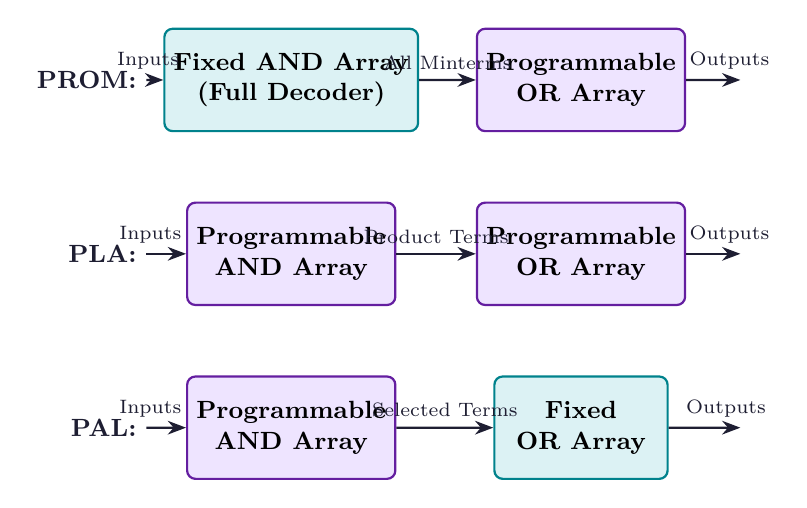
\begin{tikzpicture}[scale=0.92]
  % PROM
  \node[sysblock, draw=myteal, fill=hdrteal] (p1) at (0, 2.4) {Fixed AND Array\\(Full Decoder)};
  \node[sysblock, draw=mypurple, fill=hdrpurple] (p2) at (4.0, 2.4) {Programmable\\OR Array};
  \draw[flowarrow] (-2.0, 2.4) -- (p1) node[pos=0.1, above, font=\scriptsize] {Inputs};
  \draw[flowarrow] (p1) -- (p2) node[midway, above, font=\scriptsize] {All Minterms};
  \draw[flowarrow] (p2) -- (6.2, 2.4) node[pos=0.8, above, font=\scriptsize] {Outputs};
  \node[left, font=\small\bfseries\color{mydark}] at (-2.0, 2.4) {PROM:};

  % PLA
  \node[sysblock, draw=mypurple, fill=hdrpurple] (pa1) at (0, 0) {Programmable\\AND Array};
  \node[sysblock, draw=mypurple, fill=hdrpurple] (pa2) at (4.0, 0) {Programmable\\OR Array};
  \draw[flowarrow] (-2.0, 0) -- (pa1) node[pos=0.1, above, font=\scriptsize] {Inputs};
  \draw[flowarrow] (pa1) -- (pa2) node[midway, above, font=\scriptsize] {Product Terms};
  \draw[flowarrow] (pa2) -- (6.2, 0) node[pos=0.8, above, font=\scriptsize] {Outputs};
  \node[left, font=\small\bfseries\color{mydark}] at (-2.0, 0) {PLA:};

  % PAL
  \node[sysblock, draw=mypurple, fill=hdrpurple] (pl1) at (0, -2.4) {Programmable\\AND Array};
  \node[sysblock, draw=myteal, fill=hdrteal] (pl2) at (4.0, -2.4) {Fixed\\OR Array};
  \draw[flowarrow] (-2.0, -2.4) -- (pl1) node[pos=0.1, above, font=\scriptsize] {Inputs};
  \draw[flowarrow] (pl1) -- (pl2) node[midway, above, font=\scriptsize] {Selected Terms};
  \draw[flowarrow] (pl2) -- (6.2, -2.4) node[pos=0.8, above, font=\scriptsize] {Outputs};
  \node[left, font=\small\bfseries\color{mydark}] at (-2.0, -2.4) {PAL:};
\end{tikzpicture}
\end{tcolorbox}

\subsection{Complex Programmable Logic Devices (CPLD)}
A CPLD integrates multiple PAL/GAL-like \textbf{Function Blocks (Logic Array Blocks)} interconnected through a centralized, uniform \textbf{Global Interconnect Matrix (GIM)}.
\begin{itemize}[leftmargin=*, itemsep=3pt]
  \item Features non-volatile EEPROM/Flash configuration storage (starts up instantly upon power application).
  \item Delivers predictable, deterministic pin-to-pin propagation timing delays.
  \item Typically contains tens to hundreds of macrocells (equivalent to $1{,}000$ to $100{,}000$ logic gates).
\end{itemize}

\subsection{Field Programmable Gate Arrays (FPGA)}
FPGAs are high-density digital ICs based on an \textbf{island-style architecture} consisting of a two-dimensional matrix of programmable logic resources:
\begin{itemize}[leftmargin=*, itemsep=4pt]
  \item \textbf{Configurable Logic Blocks (CLBs):} The fundamental computational building blocks. Each CLB contains:
    \begin{itemize}
      \item \textbf{Look-Up Tables (LUTs):} A $k$-input LUT is a small high-speed SRAM block ($2^k \times 1$) that implements \textbf{any arbitrary Boolean logic function of $k$ variables} simply by loading the function's truth table truth bits into memory. The inputs serve as address lines selecting the precomputed output bit.
      \item \textbf{Storage Elements:} Configurable D flip-flops / latches with clock enables, set/reset lines.
      \item \textbf{Arithmetic Carry Logic:} Dedicated ultra-fast lookahead carry chains for high-speed addition.
      \item \textbf{Multiplexers:} Wide multiplexers for combining multiple LUT outputs.
    \end{itemize}
  \item \textbf{Programmable Interconnects:} Segmented horizontal and vertical routing channels joined at programmable \textbf{Switch Boxes} and \textbf{Connection Boxes}.
  \item \textbf{Input/Output Blocks (IOBs):} Configurable bidirectional input/output buffers surrounding the periphery, supporting multiple I/O standards (LVTTL, LVCMOS, differential signaling).
  \item \textbf{Specialized Hardware Blocks:} Modern FPGAs embed dedicated DSP slices (hardwired MAC units), dual-port block RAMs (BRAM), PLLs/DCMs, and high-speed transceivers.
\end{itemize}

\par\vspace{6pt}\noindent
\begingroup
\setlength{\tabcolsep}{3.5pt}
\setlength{\extrarowheight}{3pt}
\begin{tabularx}{\linewidth}{|B{2.8cm}|Y|Y|}
\hline
\textbf{Feature} & \textbf{CPLD} & \textbf{FPGA} \\
\hline
Architecture & Coarse-grained (PAL-like function blocks) & Fine-grained (2D array of CLBs and LUTs) \\
\hline
Configuration Memory & Non-volatile (Internal Flash/EEPROM) & Volatile (SRAM-based, requires boot ROM) \\
\hline
Boot-up Time & Instant-on upon power application & Requires configuration bitstream loading \\
\hline
Interconnect & Global interconnect matrix (Centralized) & Segmented channels and switch matrices \\
\hline
Timing Predictability & Deterministic, fixed pin-to-pin delay & Variable, placement and routing dependent \\
\hline
Density / Logic Capacity & Low to moderate ($< 10{,}000$ macrocells) & Extremely High (Millions of system gates) \\
\hline
Typical Applications & Glue logic, boot controllers, address decoders & DSP, telecommunications, AI acceleration, ASIC prototyping \\
\hline
\end{tabularx}
\endgroup

% ===============================================================================
\section{Digital-to-Analog Converters (DAC)}
% ===============================================================================

A DAC translates an $n$-bit binary digital word $D = b_1 2^{-1} + b_2 2^{-2} + \dots + b_n 2^{-n}$ into a proportional analog voltage or current.

\subsection{DAC Specifications}
\begin{itemize}[leftmargin=*, itemsep=3pt]
  \item \textbf{Resolution:} The number of input bits ($n$), or the smallest output voltage increment (step size):
  \begin{equation}
    \text{Step Size} = \frac{V_{FS}}{2^n - 1} \approx \frac{V_{\text{ref}}}{2^n}
  \end{equation}
  \item \textbf{Settling Time:} The time elapsed from an input code transition until the analog output settles to within $\pm \frac{1}{2}\text{ LSB}$ of its final value.
  \item \textbf{Linearity Errors:} Integral Non-Linearity (INL) and Differential Non-Linearity (DNL).
  \item \textbf{Monotonicity:} A DAC is monotonic if its output voltage never decreases when the input digital code increases.
\end{itemize}

\subsection{Binary-Weighted Resistor DAC}
Uses an inverting operational amplifier summing configuration with binary-weighted input resistors:
\begin{equation}
  R_1 = R, \quad R_2 = 2R, \quad R_3 = 4R, \quad \dots, \quad R_n = 2^{n-1}R
\end{equation}
The output analog voltage is given by:
\begin{equation}
  V_o = -I_T R_f = -V_{\text{ref}} \frac{R_f}{R} \left( \frac{b_1}{2^1} + \frac{b_2}{2^2} + \frac{b_3}{2^4} + \dots + \frac{b_n}{2^n} \right)
\end{equation}
\textbf{Major Drawbacks:}
\begin{enumerate}[label=\arabic*., leftmargin=*]
  \item \textbf{Wide Range of Resistance Values:} For an 8-bit DAC, the resistor ratio is $2^7 : 1 = 128 : 1$; for a 16-bit DAC, it reaches $32{,}768 : 1$.
  \item Extremely difficult to fabricate widely disparate, tightly matched resistors with identical temperature coefficients on an integrated circuit die.
  \item The MSB resistor ($R$) draws significantly higher current than the LSB resistor, causing uneven thermal dissipation.
\end{enumerate}

\subsection{\texorpdfstring{$R\text{-}2R$}{R-2R} Ladder DAC}
The $R\text{-}2R$ ladder DAC overcomes all drawbacks of the binary-weighted design by requiring \textbf{only two distinct resistor values ($R$ and $2R$)} regardless of resolution $n$.

\begin{tcolorbox}[defbox, title={\textbf{Thevenin Resistance Principle of the $R\text{-}2R$ Ladder}}]
At every ladder node, the equivalent resistance looking toward the terminating end or down any branch is always exactly $R$. At each junction, the incoming current splits evenly in half ($50\%$ down the branch through $2R$, and $50\%$ onward through $R$).
\end{tcolorbox}

\begin{tcolorbox}[tikzbox, title={4-Bit $R\text{-}2R$ Ladder DAC Circuit Architecture}]
\centering
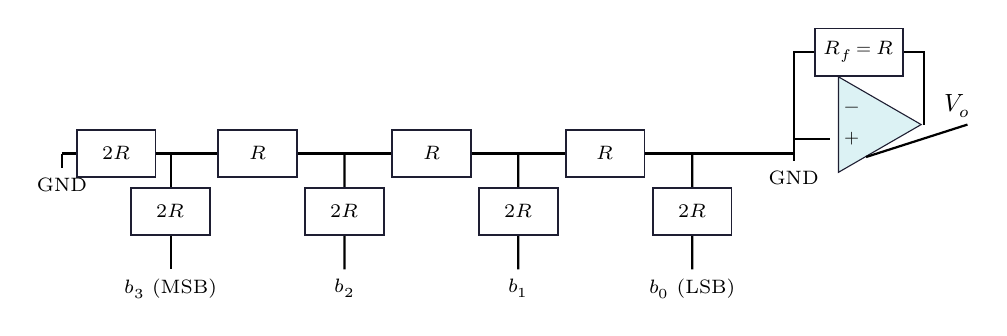
\begin{tikzpicture}[scale=0.92]
  % Nodes
  \coordinate (n3) at (0, 0);
  \coordinate (n2) at (2.4, 0);
  \coordinate (n1) at (4.8, 0);
  \coordinate (n0) at (7.2, 0);

  % Horizontal Resistors R
  \draw[thick] (-1.5, 0) -- (n3);
  \node[resnode] at (-0.75, 0) {$2R$};
  \node[below, font=\scriptsize] at (-1.5, -0.2) {GND};
  \draw[thick] (-1.5, 0) -- (-1.5, -0.2);

  \draw[thick] (n3) -- (n2);
  \node[resnode] at (1.2, 0) {$R$};

  \draw[thick] (n2) -- (n1);
  \node[resnode] at (3.6, 0) {$R$};

  \draw[thick] (n1) -- (n0);
  \node[resnode] at (6.0, 0) {$R$};

  % Vertical Resistors 2R
  \draw[thick] (n3) -- (0, -1.6);
  \node[resnode] at (0, -0.8) {$2R$};
  \node[below, font=\scriptsize] at (0, -1.6) {$b_3$ (MSB)};

  \draw[thick] (n2) -- (2.4, -1.6);
  \node[resnode] at (2.4, -0.8) {$2R$};
  \node[below, font=\scriptsize] at (2.4, -1.6) {$b_2$};

  \draw[thick] (n1) -- (4.8, -1.6);
  \node[resnode] at (4.8, -0.8) {$2R$};
  \node[below, font=\scriptsize] at (4.8, -1.6) {$b_1$};

  \draw[thick] (n0) -- (7.2, -1.6);
  \node[resnode] at (7.2, -0.8) {$2R$};
  \node[below, font=\scriptsize] at (7.2, -1.6) {$b_0$ (LSB)};

  % Op-amp Summing stage
  \draw[thick] (n0) -- (8.6, 0) -- (8.6, 0.6);
  \node[draw=mydark, fill=hdrteal, regular polygon, regular polygon sides=3, rotate=-90, minimum size=1.4cm] (opamp) at (9.6, 0.4) {};
  \node[font=\scriptsize] at (9.4, 0.6) {$-$};
  \node[font=\scriptsize] at (9.4, 0.2) {$+$};
  \draw[thick] (9.1, 0.2) -- (8.6, 0.2) -- (8.6, -0.1);
  \node[below, font=\scriptsize] at (8.6, -0.1) {GND};

  \draw[thick] (opamp.east) -- (11.0, 0.4) node[pos=0.9, above, font=\small] {$V_o$};
  \draw[thick] (8.6, 0.6) -- (8.6, 1.4) -- (10.4, 1.4) -- (10.4, 0.4);
  \node[resnode] at (9.5, 1.4) {$R_f = R$};
\end{tikzpicture}
\end{tcolorbox}

For an $n$-bit $R\text{-}2R$ ladder DAC, the analog output voltage is:
\begin{equation}
  V_o = -V_{\text{ref}} \frac{R_f}{R} \sum_{i=1}^{n} \frac{b_i}{2^i} = -V_{\text{ref}} \left( \frac{b_1}{2} + \frac{b_2}{4} + \dots + \frac{b_n}{2^n} \right) \quad (\text{when } R_f = R)
\end{equation}
\textbf{Key Advantages:}
\begin{itemize}[leftmargin=*, itemsep=2pt]
  \item Requires only two values: $R$ and $2R$.
  \item Highly practical for monolithic semiconductor IC fabrication using thin-film laser-trimmed resistors.
  \item Easily scalable to high bit-resolutions ($12$, $16$, or $24$ bits).
\end{itemize}

% ===============================================================================
\section{Analog-to-Digital Converters (ADC)}
% ===============================================================================

An ADC converts a continuous-time, continuous-amplitude analog voltage $V_{in}$ into a discrete $n$-bit digital code via three sequential steps: \textbf{Sampling, Quantization, and Binary Encoding}.

\subsection{Quantization Error and ADC Dynamic Range}
The ideal quantization step size is $\Delta = \frac{V_{FS}}{2^n - 1}$. The maximum inherent quantization uncertainty is:
\begin{equation}
  Q_e = \pm \frac{\Delta}{2}
\end{equation}
The theoretical Signal-to-Quantization-Noise Ratio (SQNR) for a full-scale sinusoidal input is:
\begin{equation}
  \text{SQNR} = 6.02 n + 1.76 \text{ dB}
\end{equation}
Every added bit of resolution improves dynamic range by approximately $6\text{ dB}$.

\subsection{Flash (Simultaneous / Parallel) ADC}
The Flash ADC is the \textbf{fastest possible ADC architecture}.
\begin{itemize}[leftmargin=*, itemsep=3pt]
  \item \textbf{Architecture:} Contains a precision reference voltage divider of $2^n$ identical resistors generating $2^n - 1$ reference thresholds, $2^n - 1$ analog comparators operating in parallel, and a priority encoder.
  \item \textbf{Operation:} All $2^n - 1$ comparators simultaneously compare $V_{in}$ against their assigned reference levels in a single clock cycle, generating a thermometer code which is converted to binary by the priority encoder.
  \item \textbf{Conversion Time:} Strictly $1$ clock cycle ($O(1)$ time complexity, typically $< 1\text{--}5\text{ ns}$).
  \item \textbf{Limitation:} Circuit hardware grows exponentially ($2^n - 1$ comparators). An 8-bit Flash ADC requires $255$ comparators; a 10-bit converter requires $1{,}023$ comparators, resulting in huge silicon area and excessive power consumption.
\end{itemize}

\subsection{Successive Approximation Register (SAR) ADC}
The SAR ADC utilizes a \textbf{binary search algorithm} to systematically approximate the input voltage bit by bit from MSB down to LSB using a single comparator and an internal DAC.
\begin{enumerate}[label=\arabic*., leftmargin=*]
  \item \textbf{Cycle 1:} The SAR sets the MSB ($b_1 = 1$, all others $0$). The DAC generates $V_{\text{DAC}} = \frac{1}{2} V_{\text{ref}}$.
  \item If $V_{in} > V_{\text{DAC}}$, the comparator output is HIGH; the MSB is retained ($b_1 = 1$). If $V_{in} < V_{\text{DAC}}$, the MSB is cleared ($b_1 = 0$).
  \item \textbf{Cycle 2 to $n$:} The process is repeated sequentially for each successive bit ($b_2, b_3, \dots, b_n$).
  \item \textbf{Conversion Time:} Strictly constant and directly proportional to resolution:
  \begin{equation}
    T_C = n \times T_{\text{clk}}
  \end{equation}
  \item \textbf{Applications:} The industry standard for medium-to-high speed ($100\text{ kSPS}$ to $10\text{ MSPS}$), $10\text{--}18\text{ bit}$ instrumentation, biomedical data acquisition (ECG/EEG), and microcontroller embedded ADCs.
\end{enumerate}

\subsection{Dual-Slope Integrating ADC}
The Dual-Slope ADC provides the \textbf{highest accuracy and superior noise rejection} through continuous analog integration.

\begin{tcolorbox}[defbox, title={\textbf{Dual-Slope Conversion Derivation}}]
\begin{itemize}[leftmargin=*, itemsep=3pt]
  \item \textbf{Phase 1 (Fixed-Time Run-Up):} Switch connects to $V_{in}$ for a fixed time $T_1 = 2^n \times T_{\text{clk}}$. The integrator output ramps to a peak voltage:
  \begin{equation}
    V_{\text{peak}} = -\frac{1}{RC} \int_{0}^{T_1} V_{in} \, dt = -\frac{V_{in} T_1}{RC}
  \end{equation}
  \item \textbf{Phase 2 (Variable-Time Run-Down):} Switch connects to a negative reference $-V_{\text{ref}}$. The integrator ramps back toward zero at a constant slope:
  \begin{equation}
    V_o(t) = V_{\text{peak}} + \frac{V_{\text{ref}} t}{RC}
  \end{equation}
  When $V_o(t) = 0$ at time $t = T_2$, the comparator stops the digital counter.
  \item Equating integrator charges:
  \begin{equation}
    \frac{V_{in} T_1}{RC} = \frac{V_{\text{ref}} T_2}{RC} \implies T_2 = T_1 \left(\frac{V_{in}}{V_{\text{ref}}}\right)
  \end{equation}
\end{itemize}
\end{tcolorbox}

\textbf{Outstanding Advantages:}
\begin{itemize}[leftmargin=*, itemsep=2pt]
  \item \textbf{Immune to Component Drift:} Conversion time $T_2$ is \textbf{entirely independent of the integration resistance $R$, capacitance $C$, and clock frequency $f_{\text{clk}}$} because they cancel out completely in the ratio.
  \item \textbf{Power-Line Noise Rejection:} By setting integration period $T_1$ to an exact integer multiple of the $50\text{ Hz}$ or $60\text{ Hz}$ power-line cycle ($20\text{ ms}$ or $16.67\text{ ms}$), hum and line noise integrate to identically zero.
  \item \textbf{Limitation:} Very slow conversion ($T_{C(\max)} = 2 \times 2^n \times T_{\text{clk}}$). Standard choice for precision Digital Multimeters (DMMs) and digital weigh scales.
\end{itemize}

\par\vspace{6pt}\noindent
\begingroup
\setlength{\tabcolsep}{3.5pt}
\setlength{\extrarowheight}{3pt}
\begin{tabularx}{\linewidth}{|B{2.2cm}|Y|Y|Y|Y|}
\hline
\textbf{Parameter} & \textbf{Flash ADC} & \textbf{SAR ADC} & \textbf{Dual-Slope ADC} & \textbf{Counter / Ramp ADC} \\
\hline
Conversion Speed & Extremely Fast ($1\text{--}5\text{ ns}$) & Fast ($1\text{--}10\,\mu\text{s}$) & Extremely Slow ($10\text{--}100\text{ ms}$) & Slow (Variable) \\
\hline
Clock Cycles & $1$ clock cycle ($O(1)$) & $n$ clock cycles & Up to $2 \times 2^n$ cycles & Up to $2^n$ cycles \\
\hline
Resolution & $6\text{--}8$ bits & $8\text{--}18$ bits & $16\text{--}24$ bits (Highest) & $8\text{--}10$ bits \\
\hline
Hardware Cost & High ($2^n - 1$ comparators) & Moderate ($1$ comp, $1$ DAC) & Low ($1$ integrator, $1$ comp) & Low ($1$ counter, $1$ DAC) \\
\hline
Noise Immunity & Poor & Moderate & Exceptional ($50/60\text{ Hz}$ hum) & Poor \\
\hline
Typical Uses & Radar, oscilloscopes, video & Microcontrollers, DSP & DMMs, weighing scales & Low-cost sensors \\
\hline
\end{tabularx}
\endgroup

% ===============================================================================
\section{Sample and Hold (S/H) Circuit}
% ===============================================================================

When converting high-frequency analog signals, any input variation during the finite conversion interval ($t_c$) introduces \textbf{aperture error}. A Sample-and-Hold circuit freezes the analog voltage for the duration of the ADC conversion.

\subsection{Circuit Topology and Modes of Operation}
A basic S/H circuit consists of an input unity-gain buffer op-amp, a high-speed analog switch (JFET or MOSFET), an ultra-low leakage \textbf{Hold Capacitor ($C_H$)}, and an output high-input-impedance unity-gain buffer op-amp.
\begin{itemize}[leftmargin=*, itemsep=3pt]
  \item \textbf{Sample (Track) Mode:} The switch is closed (ON). The hold capacitor $C_H$ charges to follow the input analog voltage $V_{in}$ through the switch ON resistance $R_{\text{on}}$.
  \item \textbf{Hold Mode:} The switch is opened (OFF). The charge trapped on $C_H$ maintains the instantaneous voltage constant. The high-impedance buffer delivers this stable voltage to the ADC.
\end{itemize}

\subsection{Key Dynamic Performance Parameters}
\begin{itemize}[leftmargin=*, itemsep=3pt]
  \item \textbf{Acquisition Time ($t_{ac}$):} Time required for the hold capacitor voltage to charge and settle to within a specified error band (e.g., $0.01\%$ or $\pm \frac{1}{2}\text{ LSB}$) following a transition from hold to sample mode. Governed by switch resistance and capacitance:
  \begin{equation}
    t_{ac} \approx k \cdot R_{\text{on}} \cdot C_H \quad (\text{where } k \approx 7\text{--}9 \text{ for 12-bit accuracy})
  \end{equation}
  \item \textbf{Aperture Time ($t_{ap}$):} The finite delay between the initiation of the hold command and the effective physical opening of the sampling switch.
  \item \textbf{Aperture Jitter ($t_j$):} The sample-to-sample statistical timing uncertainty in switch opening. The maximum input signal frequency before aperture jitter exceeds $1\text{ LSB}$ is:
  \begin{equation}
    f_{\max} = \frac{1}{2\pi \cdot t_j \cdot 2^n}
  \end{equation}
  \item \textbf{Droop Rate ($\frac{dV}{dt}$):} The rate at which the output voltage drifts during hold mode due to capacitor discharge through parasitic leakage currents:
  \begin{equation}
    \text{Droop Rate} = \frac{I_{\text{leak}}}{C_H}
  \end{equation}
  \item \textbf{Trade-off in Sizing $C_H$:} A large $C_H$ reduces droop rate but increases acquisition time; a small $C_H$ accelerates acquisition but degrades droop performance.
\end{itemize}

\newpage
% ===============================================================================
\section{Quick Revision Page}
% ===============================================================================

\begin{tcolorbox}[formulabox, title={\textbf{Key Formulas and Characteristic Relations at a Glance}}]
\begin{itemize}[leftmargin=*, itemsep=3pt]
  \item \textbf{Digital IC Speed-Power Metric:}
  \begin{equation*}
    t_{pd} = \frac{t_{PLH} + t_{PHL}}{2}, \quad \text{PDP} = P_D \times t_{pd}, \quad P_{\text{dyn(CMOS)}} = \alpha C_L V_{DD}^2 f
  \end{equation*}
  \item \textbf{Noise Margins and Open-Collector Pull-up Resistor:}
  \begin{equation*}
    NM_H = V_{OH(\min)} - V_{IH(\min)}, \quad NM_L = V_{IL(\max)} - V_{OL(\max)}, \quad R_{P(\min)} = \frac{V_{CC} - V_{OL}}{I_{OL} - N \cdot I_{IL}}
  \end{equation*}
  \item \textbf{DAC Resolution and Analog Output ($R\text{-}2R$ Ladder):}
  \begin{equation*}
    \text{Step Size} = \frac{V_{FS}}{2^n - 1}, \quad V_o = -V_{\text{ref}} \left(\frac{b_1}{2} + \frac{b_2}{4} + \dots + \frac{b_n}{2^n}\right)
  \end{equation*}
  \item \textbf{ADC Timing and Dual-Slope Relation:}
  \begin{equation*}
    T_{C(\text{SAR})} = n \cdot T_{\text{clk}}, \quad T_{C(\text{Flash})} = 1 \cdot T_{\text{clk}}, \quad T_2 = T_1 \cdot \left(\frac{V_{in}}{V_{\text{ref}}}\right)
  \end{equation*}
\end{itemize}
\end{tcolorbox}

\begin{tcolorbox}[defbox, title={\textbf{One-Line High-Yield Definitions}}]
\begin{itemize}[leftmargin=*, itemsep=2pt]
  \item \textbf{Noise Margin:} The maximum noise voltage amplitude that can be added to an input signal without corrupting the recognized logic level.
  \item \textbf{Totem-Pole Output:} An active BJT push-pull output driver providing low impedance during both pull-up and pull-down transitions.
  \item \textbf{ECL Logic Family:} Non-saturating BJT current-steering logic that avoids saturation charge storage to achieve sub-nanosecond speeds.
  \item \textbf{Static RAM (SRAM):} Volatile memory storing data in bi-stable cross-coupled CMOS inverters requiring no periodic refresh.
  \item \textbf{Dynamic RAM (DRAM):} Volatile memory storing data as charge on a 1T-1C capacitor requiring periodic refresh cycles.
  \item \textbf{Look-Up Table (LUT):} An SRAM-based truth table in an FPGA that realizes any arbitrary $k$-variable logic function.
  \item \textbf{Flash ADC:} A parallel ADC utilizing $2^n - 1$ simultaneous comparators to perform conversions in a single clock cycle.
  \item \textbf{Dual-Slope ADC:} An integrating ADC whose conversion is independent of $R$, $C$, and clock frequency, offering high noise rejection.
  \item \textbf{SAR ADC:} An analog-to-digital converter that determines binary bits sequentially via a binary search algorithm in $n$ cycles.
  \item \textbf{Droop Rate:} The rate of voltage decay across the hold capacitor in a Sample-and-Hold circuit caused by parasitic leakage.
\end{itemize}
\end{tcolorbox}

\begin{tcolorbox}[exambox, title={\textbf{Frequently Asked / Viva Questions}}]
\begin{enumerate}[label=\arabic*., leftmargin=*]
  \item \Q{Why can totem-pole TTL outputs not be connected in a wired-AND configuration?}
  If one gate asserts HIGH and the other LOW, a direct low-resistance short circuit from $V_{CC}$ to ground through $Q_3$ and $Q_4$ occurs, producing damaging current spikes and destruction.

  \item \Q{Why is ECL significantly faster than TTL?}
  ECL operates BJTs strictly in the non-saturating active region using a differential current-steering switch. Eliminating saturation eliminates base minority carrier storage time ($t_s = 0$).

  \item \Q{Why does static CMOS consume virtually zero power at DC?}
  For any stable logic input, either the PMOS pull-up network or the NMOS pull-down network is completely turned OFF, cutting off any direct path between $V_{DD}$ and ground.

  \item \Q{Why must PMOS transistors be made wider than NMOS in CMOS inverters?}
  Because electron mobility in silicon is approximately $2.5$ times higher than hole mobility ($\mu_n \approx 2.5 \mu_p$). PMOS width must be scaled by $2.5\times$ to equalize drive currents.

  \item \Q{Why does DRAM require periodic refreshing while SRAM does not?}
  DRAM stores data as charge on tiny capacitors ($C_s \approx 30\text{ fF}$) which leak through semiconductor junctions within milliseconds. SRAM uses cross-coupled active latching inverters.

  \item \Q{Explain the functional architectural difference between PLA and PAL.}
  A PLA features both programmable AND and programmable OR arrays, offering maximum term sharing. A PAL has a programmable AND array and a fixed OR array, offering faster speed and simpler structure.

  \item \Q{What is a Look-Up Table (LUT) in an FPGA?}
  An LUT is a small SRAM block storing the truth table values of a logic function. For a 4-input LUT, 4 input lines act as addresses selecting 1 of 16 stored output bits.

  \item \Q{Why is an $R\text{-}2R$ ladder DAC preferred over a binary-weighted resistor DAC?}
  An $R\text{-}2R$ ladder requires only two resistor values ($R$ and $2R$) regardless of bit resolution, avoiding the fabrication of massive, tightly matched resistor ranges.

  \item \Q{How many comparators are required for an 8-bit Flash ADC?}
  An 8-bit Flash ADC requires $2^8 - 1 = 255$ parallel comparators.

  \item \Q{Why is conversion time constant in a SAR ADC regardless of input voltage?}
  Because a SAR ADC always executes a fixed $n$-step binary search sequence, testing one bit per clock cycle from MSB to LSB.

  \item \Q{Why is the Dual-Slope ADC immune to variations in resistance and capacitance?}
  Because the integrator component values $R$ and $C$ appear identically in both the run-up and run-down equations and cancel out completely in the ratio $T_2 = T_1 (V_{in}/V_{\text{ref}})$.

  \item \Q{What causes aperture jitter in a Sample-and-Hold circuit, and why is it problematic?}
  Aperture jitter is the sample-to-sample statistical variation in the switch opening moment, which introduces phase noise and voltage errors when sampling fast-changing analog signals.
\end{enumerate}
\end{tcolorbox}

\begin{tcolorbox}[tikzbox, title={\textbf{Summary Matrix: Comparison of ADC Architectures}}]
\centering
\begingroup
\setlength{\tabcolsep}{4pt}
\setlength{\extrarowheight}{3pt}
\begin{tabularx}{\linewidth}{|B{3.2cm}|Y|Y|Y|}
\hline
\textbf{Metric} & \textbf{Flash ADC} & \textbf{SAR ADC} & \textbf{Dual-Slope ADC} \\
\hline
Conversion Time ($T_C$) & $1$ clock cycle ($O(1)$) & $n$ clock cycles ($O(n)$) & Up to $2^{n+1}$ cycles ($O(2^n)$) \\
\hline
Relative Speed & Ultra-fast ($> 1\text{ GSPS}$) & Medium-high ($100\text{ kSPS}$--$10\text{ MSPS}$) & Very slow ($10$--$100\text{ SPS}$) \\
\hline
Hardware Complexity & Exponential ($2^n - 1$ comparators) & Moderate ($1$ comp, $1$ DAC, SAR) & Minimal ($1$ integrator, $1$ comp) \\
\hline
Resolution Limits & $6\text{--}8$ bits (rarely 10) & $8\text{--}18$ bits & $16\text{--}24$ bits (Extreme precision) \\
\hline
Noise Rejection & Poor & Moderate & Superb (line hum canceling) \\
\hline
Dominant Usage & Oscilloscopes, SDR, radar & Embedded MCUs, audio, DSP & Digital multimeters, scales \\
\hline
\end{tabularx}
\endgroup
\end{tcolorbox}

\end{document}
